\subsection{Overview}

\begin{figure*}
    \centering
    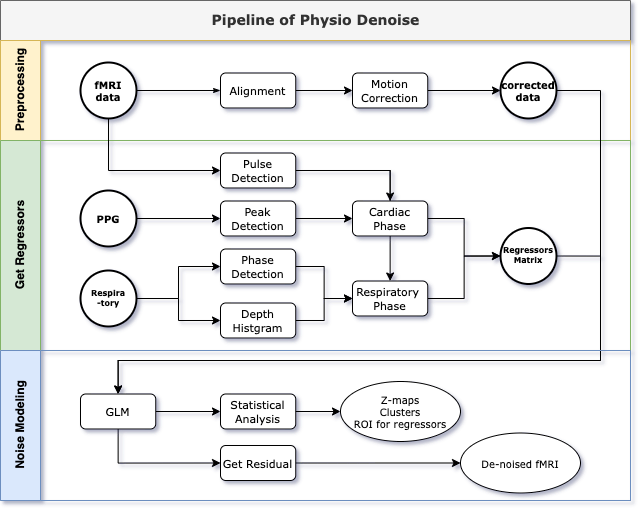
\includegraphics[width=0.8\textwidth]{Figures/pipe.png}
    \caption{Workflow of Physio Denoise}
    \label{fig:modules}
\end{figure*} 

Physio Denoise consists of three main modules, as depicted in Fig. \ref{fig:modules}, 
including preprocessing of fMRI data, preprocessing of physiological data  and noise modeling.
Briefly, the first module preprocesses the raw fMRI data with motion correction, 
and the second module deals with physiological data and generate regressors
from these data. 
These two modules prepare the basic materials for the noise model. 
Exploiting the idea of RETROICOR model, 
noise modeling module uses prepared regressors to build a GLM.
Physiological regressors are used as independent variables in the model. 
So when regressing out all the physiological components, a cleaned fMRI data could be gained. 

The compulsory inputs for this tool include a raw fMRI data, 
physiological signals which should be saved in text file in which three columns respectively stand for cardiac signal, 
respiration signal and time stamps,
TR time, sample rate and working directory.

\subsection{Software and Packages}

(Introduction of needed tools, to be continued.)

\textbf{FSL},

\textbf{Nilearn},


\textbf{HeartPy}\cite{van2019heartpy},

\textbf{Neurokit2}\cite{Makowski2021neurokit},

\textbf{Click},


\subsection{Data Preprocessing}

Although Physio Denoise is used for denoising, the preprocessing of fMRI data is still essential.
The preprocessing pipeline consists of alignment and motion correction.
% , as it shown in Fig.
% \ref{fig:graph}.

Alignment chooses the middle volume from the whole fMRI data as reference, and registers the other
volumes to it. 

The main idea of motion correction is to correct the bulk motion noise. 
But different from the respiratory motion of breathing, this motion correction
is mainly bulk motion caused by subjects' movement. During the scan, motion noise is inevitable. 
Keeping subjects completely still during the whole scan is impractical.
Although small breaks are usually designed between each task during the scan in order to let subjects relax themselves, 
behaviors like swallowing and blinking still exist.
Bulk motion can have large effects on activation maps for analysis, 
which usually occur at edges in the image; 
this is due to the fact that large changes in image intensity can occur 
when a voxel that has no brain tissue in it at one point 
suddenly contains tissue due to motion. \cite{poldrack2011handbook}


% \begin{figure}[htp]
%     \centering
%     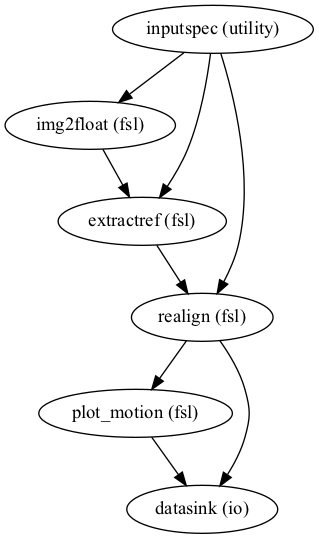
\includegraphics[width=0.7\columnwidth]{Figures/gragh.png}
%     \caption{The pipeline of preprocessing of fMRI data}
%     \label{fig:graph}
% \end{figure}

In order to model the physiological noise model more precisely, 
this step aims to clean the raw data roughly as the first step.
In the whole motion noise, we still couldn't find a clear boundary
to separate physiological noise and noise from purely movement, but a motion correction could
still help with the specificity in noise modeling. And the correction in 6 degree will be plotted 
as results.

\subsection{Processing of Physiological data}
The main idea of processing physiological data is to extract needed regressors for the noise model.

\subsubsection{Scan Time Detection}
The whole denoising process aims at correcting fMRI data for each scan. 
So the time stamp of the beginning of each scan could be used to represent each volume image. 
Using scan time detection part also synchronizes physiological signals to each volume in fMRI data,
which is essential to get regressors in the modeling part.

Segmentation is also applied on input physiological data which
limits the length of signals to be consistent with fMRI data. 
Because during the data acquisition, the physiological
data is usually collected by external equipments such as Biopac rather than MRI device, 
length of signals may not be the same. Moreover, as mentioned in the background, the respiratory phase calculation 
partly depends on the histogram of the amplitude during the whole scan. So an incompatible length of 
respiratory signal might influence the phase values which indirectly effects the noise model. To be specific, 
a period of unexpected unstable signal could be accidentally collected when subjects taking off the 
device, which may change the distribution of histogram in a way.

After scan time detection, the length of physiological signals will be limited to be 3 TR time longer than the 
fMRI data. And a csv file recording each scan time will be generated in the working directory.

\subsubsection{Cardiac Regressors}

In Physio Denoise, we choose a less invasive method of assessing cardiac cycles, which is Photoplethysmogram (PPG). 
PPG devices employ an optical sensor to measure the changes in coloration of the skin as blood perfuses through the arteries and capillaries with each heartbeat. \cite{van2019heartpy}

With the help of HeartPy, the peak of the signal could be detected and marked, as it shows in Fig. \ref{fig:heart}

\begin{figure}[htp]
    \centering
    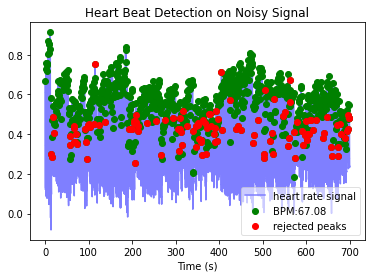
\includegraphics[width=\columnwidth]{Figures/heartpy.png}
    \caption{An example of PPG signal analyzed by HeartPy. The green points represent the accepted peaks,
    while the red points are rejected by HeartPy. Peaks are considered low confidence if the interval created between two adjacent peaks deviates 
    by more than 30\% of the mean peak-peak interval of the analyzed segment. \cite{van2019heartpy}}
    \label{fig:heart}
\end{figure} 

\begin{figure}[htp]
    \centering
    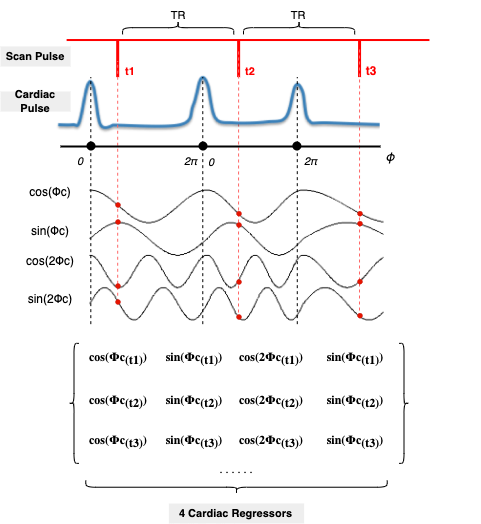
\includegraphics[width=\columnwidth]{Figures/cardiac.png}
    \caption{After detecting the peak in cardiac signal, the cardiac regressors from a second order Fourier expanded formula are generated with three MRI time stamps. 
    The matrix represents the way regressors constructing the independent variables $X$ in GLM }
    \label{fig:cardiac}
\end{figure} 

While a sequence of peaks from PPG signal is generated, 
two continuous peaks are found for the time stamp of each scan.
The scan time will locate between these two peaks. 
So that cardiac phase value in the formula \ref{eqn:cardiac} could be gained. An example of 
cardiac regressors' calculation in Fig \ref{fig:cardiac} shows the process. 
In the design of GLM, each row of variable matrix in formula \ref{eqn:glm} indicates all used regressors
for one time stamp. The number of rows equals to the number of scan.

\subsubsection{Respiration Regressors}

Respiratory signal of subjects is collected by breathing belt, which warps around chest of subjects. 
So the belt would deform with expiration and inspiration, the amplitude of signal from the 
belt is recorded as respiratory signal. 

As we introduce before, respiratory phase calculation considers both breathing state and depth.
So in this part, it divides into two parts, state analysis and value calculation.

To analyze the state of breathing, a novel tool NeuroKit2\cite{Makowski2021neurokit} is exploited 
for detection. Inspiration, expiration and implausible periods are marked by NeuroKit2. 
Similar to the way of finding cardiac phase, with time stamps from MRI data, a respiratory phase
could be easily found with results from NeuroKit2. In Fig. \ref{fig:rsp_phase}, it shows part of the 
respiratory sample as well as the phases. The curve going down indicates the expiration, which 
phase value is $-1$. On the contrary, a rising part represents inspiration with a phase value of $1$. 

\begin{figure}[htp]
    \centering
    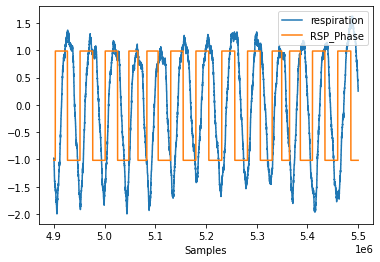
\includegraphics[width=\columnwidth]{Figures/rsp_phase.png}
    \caption{}
    \label{fig:rsp_phase}
\end{figure} 

To quantify the depth of breathe, a normalized histogram collecting all the amplitude values
shows a distribution of depth during the whole scan. 
So that at each given time stamp, its amplitude could locate the position in histogram by the normalized value in x coordinate,
which is shown in the Fig. \ref{fig:hist}. For example, when the normalized amplitude is located in 
The value for respiratory phase is gained by dividing area A by the sum of area A and B.

\begin{figure}[htp]
    \centering
    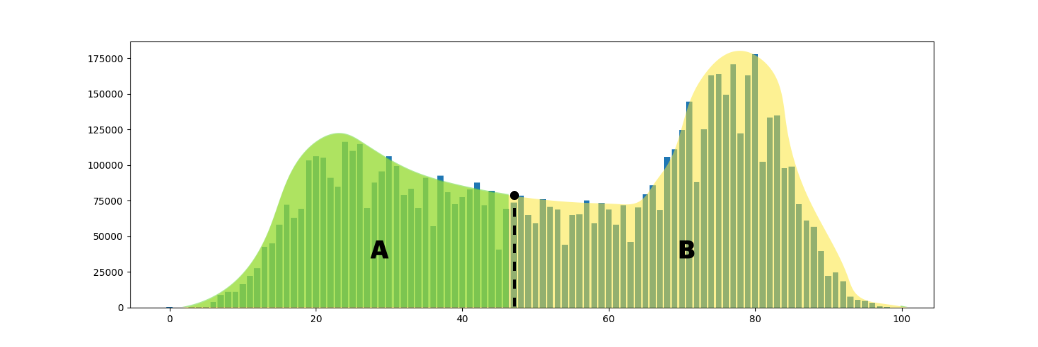
\includegraphics[width=\columnwidth]{Figures/histogram.png}
    \caption{}
    \label{fig:hist}
\end{figure}

However, the detection of breathing belt is based on physical motion that doesn't always give back
perfect data. Sometimes, the belt might be too loose or tight in measurement. The over tightness usually leads
to an abnormal amplitude that is higher than the normal range. In this work, abnormal signals will be 
kicked out before being used into the histogram.

Finally, phase value from the histogram will be given a polarity according to the state of the time.
Same as the cardiac regressors, each time stamp would have multiple regressors based 
on the Fourier expansion and its order.


\subsubsection{Noise Modeling}

Exploiting the idea of GLM, regressors from last step are independent variables in a GLM 
equation, while a preprocessed fMRI data is the dependent variable. 
To find the region of interest(ROI) of different regressor, several contrasts are built, and
each contrast represents one regressor. With the help of statistical analysis, 
Z-value maps from each contrast will show the specific region according to each regressor.
A z-map with a given threshold indicates the regions in which 
some noise signal is well explained by the according regressor.
In other words, it displays the region that physiological noise exists. 
From the statistical analysis, the area of physiological noise is plotted for all regressors.
Moreover, clusters from GLM model with ROI are extracted. With the weight values from the results of GLM model, 
temporal signals are easily constructed for ROI as well as a frequency spectrum.

% \subsection{Usage}

% The usage of Physio Denois is straightforward.
